\documentclass[tikz, border = 1 cm]{standalone}

%%%%%%%%%%%%%%
\usepackage{tikz}
\usetikzlibrary{calc}
\usetikzlibrary{positioning}
\usetikzlibrary{shapes}
%%%%%%%%%%%%%%

%%%%%%%%%%%%%%
\def\xaxis{3.5}
\def\yaxis{5}

\definecolor{blue4}{RGB}{178,231,248}
\definecolor{bluegray1}{RGB}{0,127,167}
\definecolor{bluegray2}{RGB}{76,165,193}
\definecolor{gray1}{RGB}{76,84,93}
\definecolor{gray3}{RGB}{165,169,174}
\definecolor{orange1}{RGB}{255,126,46}
\definecolor{purple}	{RGB}{89,89,171}
%%%%%%%%%%%%%%

%%%%%%%%%%%%%%
%%%%%%%%%%%%%%
%%%%%%%%%%%%%%
\begin{document}

%%%%%%%%%%%%%%
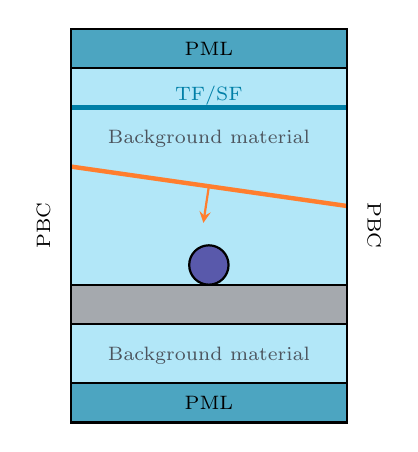
\begin{tikzpicture}

	%%% Box
	\filldraw[fill=blue4,draw=black,thick] (0,0) -- (0,\yaxis) -- (\xaxis,\yaxis) -- (\xaxis,0) -- cycle;
	
	%%% PBC nodes
	\node[rotate=90] at (-0.1*\xaxis, 0.5*\yaxis) {\scriptsize PBC};
	\node[rotate=-90] at (1.1*\xaxis, 0.5*\yaxis) {\scriptsize PBC};

	%%% PML zones
	\filldraw[fill=bluegray2,draw=black,thick] (0,0) -- (0,0.1*\yaxis) -- (\xaxis,0.1*\yaxis) -- (\xaxis,0) -- cycle;	
	\filldraw[fill=bluegray2,draw=black,thick] (0,\yaxis) -- (0,0.9*\yaxis) -- (\xaxis,0.9*\yaxis) -- (\xaxis,\yaxis) -- cycle;
	\node at (0.5*\xaxis, 0.95*\yaxis) {\scriptsize PML};
	\node at (0.5*\xaxis, 0.05*\yaxis) {\scriptsize PML};
	
	%%% TF/SF plane and node
	\draw[draw=bluegray1,ultra thick] (0,0.8*\yaxis) -- (\xaxis,0.8*\yaxis);
	\node[bluegray1] at (0.5*\xaxis, 0.83*\yaxis) {\scriptsize TF/SF};
	
	%%% Plane wave and undertermined zone
	\draw[draw=orange1,ultra thick] (0,0.65*\yaxis) -- (\xaxis,0.55*\yaxis);
	\draw[draw=orange1,thick,-stealth] (0.5*\xaxis,0.6*\yaxis) -- (0.48*\xaxis,0.507*\yaxis);
	
	%%% Object
	\filldraw[fill=gray3,draw=black,thick] (0,0.25*\yaxis) -- (0,0.35*\yaxis) -- (\xaxis,0.35*\yaxis) -- (\xaxis,0.25*\yaxis) -- cycle;	
	\filldraw[fill=purple,draw=black,thick] (0.5*\xaxis,0.4*\yaxis) circle (0.05*\yaxis);
	
	%%% Background material text
	\node[gray1] at (0.5*\xaxis, 0.72*\yaxis) {\scriptsize Background material};
	\node[gray1] at (0.5*\xaxis, 0.17*\yaxis) {\scriptsize Background material};
	
	%%% Redraw box
	\draw[draw=black,thick] (0,0) -- (0,\yaxis) -- (\xaxis,\yaxis) -- (\xaxis,0) -- cycle;
	    
\end{tikzpicture}
%%%%%%%%%%%%%%

\end{document}